% Options for packages loaded elsewhere
% Options for packages loaded elsewhere
\PassOptionsToPackage{unicode}{hyperref}
\PassOptionsToPackage{hyphens}{url}
%
\documentclass[
  ignorenonframetext,
  english,
]{beamer}
\newif\ifbibliography
\usepackage{pgfpages}
\setbeamertemplate{caption}[numbered]
\setbeamertemplate{caption label separator}{: }
\setbeamercolor{caption name}{fg=normal text.fg}
\beamertemplatenavigationsymbolsempty
% remove section numbering
\setbeamertemplate{part page}{
  \centering
  \begin{beamercolorbox}[sep=16pt,center]{part title}
    \usebeamerfont{part title}\insertpart\par
  \end{beamercolorbox}
}
\setbeamertemplate{section page}{
  \centering
  \begin{beamercolorbox}[sep=12pt,center]{section title}
    \usebeamerfont{section title}\insertsection\par
  \end{beamercolorbox}
}
\setbeamertemplate{subsection page}{
  \centering
  \begin{beamercolorbox}[sep=8pt,center]{subsection title}
    \usebeamerfont{subsection title}\insertsubsection\par
  \end{beamercolorbox}
}
% Prevent slide breaks in the middle of a paragraph
\widowpenalties 1 10000
\raggedbottom
\AtBeginPart{
  \frame{\partpage}
}
\AtBeginSection{
  \ifbibliography
  \else
    \frame{\sectionpage}
  \fi
}
\AtBeginSubsection{
  \frame{\subsectionpage}
}
\usepackage{iftex}
\ifPDFTeX
  \usepackage[T1]{fontenc}
  \usepackage[utf8]{inputenc}
  \usepackage{textcomp} % provide euro and other symbols
\else % if luatex or xetex
  \usepackage{unicode-math} % this also loads fontspec
  \defaultfontfeatures{Scale=MatchLowercase}
  \defaultfontfeatures[\rmfamily]{Ligatures=TeX,Scale=1}
\fi
\usepackage{lmodern}

\ifPDFTeX\else
  % xetex/luatex font selection
\fi
% Use upquote if available, for straight quotes in verbatim environments
\IfFileExists{upquote.sty}{\usepackage{upquote}}{}
\IfFileExists{microtype.sty}{% use microtype if available
  \usepackage[]{microtype}
  \UseMicrotypeSet[protrusion]{basicmath} % disable protrusion for tt fonts
}{}
\makeatletter
\@ifundefined{KOMAClassName}{% if non-KOMA class
  \IfFileExists{parskip.sty}{%
    \usepackage{parskip}
  }{% else
    \setlength{\parindent}{0pt}
    \setlength{\parskip}{6pt plus 2pt minus 1pt}}
}{% if KOMA class
  \KOMAoptions{parskip=half}}
\makeatother


\usepackage{longtable,booktabs,array}
\newcounter{none} % for unnumbered tables
\usepackage{calc} % for calculating minipage widths
\usepackage{caption}
% Make caption package work with longtable
\makeatletter
\def\fnum@table{\tablename~\thetable}
\makeatother
\usepackage{graphicx}
\makeatletter
\newsavebox\pandoc@box
\newcommand*\pandocbounded[1]{% scales image to fit in text height/width
  \sbox\pandoc@box{#1}%
  \Gscale@div\@tempa{\textheight}{\dimexpr\ht\pandoc@box+\dp\pandoc@box\relax}%
  \Gscale@div\@tempb{\linewidth}{\wd\pandoc@box}%
  \ifdim\@tempb\p@<\@tempa\p@\let\@tempa\@tempb\fi% select the smaller of both
  \ifdim\@tempa\p@<\p@\scalebox{\@tempa}{\usebox\pandoc@box}%
  \else\usebox{\pandoc@box}%
  \fi%
}
% Set default figure placement to htbp
\def\fps@figure{htbp}
\makeatother



\ifLuaTeX
\usepackage[bidi=basic,shorthands=off]{babel}
\else
\usepackage[bidi=default,shorthands=off]{babel}
\fi
\ifLuaTeX
  \usepackage{selnolig} % disable illegal ligatures
\fi


\setlength{\emergencystretch}{3em} % prevent overfull lines

\providecommand{\tightlist}{%
  \setlength{\itemsep}{0pt}\setlength{\parskip}{0pt}}



 


\makeatletter
\@ifpackageloaded{caption}{}{\usepackage{caption}}
\AtBeginDocument{%
\ifdefined\contentsname
  \renewcommand*\contentsname{Table of contents}
\else
  \newcommand\contentsname{Table of contents}
\fi
\ifdefined\listfigurename
  \renewcommand*\listfigurename{List of Figures}
\else
  \newcommand\listfigurename{List of Figures}
\fi
\ifdefined\listtablename
  \renewcommand*\listtablename{List of Tables}
\else
  \newcommand\listtablename{List of Tables}
\fi
\ifdefined\figurename
  \renewcommand*\figurename{Figure}
\else
  \newcommand\figurename{Figure}
\fi
\ifdefined\tablename
  \renewcommand*\tablename{Table}
\else
  \newcommand\tablename{Table}
\fi
}
\@ifpackageloaded{float}{}{\usepackage{float}}
\floatstyle{ruled}
\@ifundefined{c@chapter}{\newfloat{codelisting}{h}{lop}}{\newfloat{codelisting}{h}{lop}[chapter]}
\floatname{codelisting}{Listing}
\newcommand*\listoflistings{\listof{codelisting}{List of Listings}}
\makeatother
\makeatletter
\makeatother
\makeatletter
\@ifpackageloaded{caption}{}{\usepackage{caption}}
\@ifpackageloaded{subcaption}{}{\usepackage{subcaption}}
\makeatother

\usepackage{bookmark}
\IfFileExists{xurl.sty}{\usepackage{xurl}}{} % add URL line breaks if available
\urlstyle{same}
\hypersetup{
  pdftitle={ECN 102: Analysis of Economics Data},
  pdfauthor={Remy Beauregard},
  pdflang={en},
  hidelinks,
  pdfcreator={LaTeX via pandoc}}


\title{\texorpdfstring{ECN 102: Analysis of Economics
Data}{ECN 102: Analysis of Economics Data}}
\subtitle{\texorpdfstring{Chapter 12: Errors and
Prediction}{Chapter 12: Errors and Prediction}}
\author{Remy Beauregard}
\date{}

\begin{document}
\frame{\titlepage}


\begin{frame}{Standard Errors: Overview}
\protect\phantomsection\label{standard-errors-overview}
Our standard error for a statistic is our best estimate for the
population standard deviation of that statistic. From this measure, we
derive our inference about a population parameter from our sample
estimation. Thus, it is critical that we are using the proper standard
error for a given setting. We will think about a few cases where typical
standard errors would be inappropriate and would lead to improper
statistical inference.
\end{frame}

\begin{frame}[fragile]{Robust Standard Errors}
\protect\phantomsection\label{robust-standard-errors}
We have discussed the first case already: \textbf{robust standard
errors}. Just like in the bivariate case, we invoke robust standard
errors (with the \texttt{robust} option in Stata) to address possible
threats to homoskedasticity. However, it is common practice in Economics
to default to using robust standard errors, since our assumption of
homoskedasticity frequently is violated.

We do not worry about over-using robust standard errors, as these errors
are valid even if homoskedasticity \emph{does} hold. However, if it does
not hold, non-robust standard errors would be incorrect. Our use of
robust standard errors relaxes our third assumption to be:

\[Var[u_i|x_{2i},...,x_{ki}]=\sigma^2_{ui},\hspace{5pt} i=1,...n\]
\end{frame}

\begin{frame}{Clustered Standard Errors}
\protect\phantomsection\label{clustered-standard-errors}
In addition to being heteroskedastic, we may think that our errors may
be correlated for given sets of observations and violate independence.
In this case, we would want to \textbf{cluster} our observations by some
group variable \(G\) to address this threat to the fourth assumption.

For example, if we are studying the effect of a farm subsidy program on
household crop outcomes, we may anticipate that harvests would be
correlated for all households in a given village. In this case, we would
want to cluster our standard errors at the village level, to account for
the fact that:

\begin{enumerate}
\item
  We assume errors \emph{within} a cluster will be correlated(not
  independent)
\item
  We assume errors \emph{between} clusters will not be correlated
  (independent)
\end{enumerate}
\end{frame}

\begin{frame}{Clustered Standard Errors: Modified Assumptions}
\protect\phantomsection\label{clustered-standard-errors-modified-assumptions}
Clustering our standard errors \emph{automatically uses robust standard
errors} and changes our four population assumptions to account for the
fact that errors within clusters may be correlated but errors between
clusters should not be:

\(2_{clu}\): Cluster unbiasedness
\[E[u_i|x_{2i},...x_{ki},x_{2j},...,x_{kj}]=0\text{ for }i\text{ and }j\text{ in the same cluster}\]

\(3_{clu}\): Cluster homoskedasticity
\[Var[u_i|x_{2i},...,x_{ki}]=\sigma^2_{ui}\text{ for }i=1,...,N\]

\(4_{clu}\): Cluster independence
\[Cor[u_i,u_j|x_{2i},...,x_{ki},x_{2j},...,x_{kj}]
\begin{cases}
\neq 0 & i\text{ and }j\text{ in the same cluster}\\
= 0 & i\text{ and }j\text{ in different clusters}
\end{cases}\]
\end{frame}

\begin{frame}{Bootstrapped Standard Errors}
\protect\phantomsection\label{bootstrapped-standard-errors}
Finally, we may suspect that our data does not even fulfill linearity
(\(\hat{y}=\beta_1+\beta_2x_2+...+\beta_kx_k\)). In this case, our
estimated standard errors for \(b_1,b_2,...,b_k\) may be too large and
we need to \textbf{bootstrap}.

Bootstrapping is essentially treating our sample as the population and
resampling (with replacement) a large number of times to compute new
statistics. Then, the variation across our different bootstrap samples
gives us a ``bootstrapped'' estimate of our standard error for that
statistic.
\end{frame}

\begin{frame}{Bootstrap: Example Procedure}
\protect\phantomsection\label{bootstrap-example-procedure}
For example, if we want to bootstrap our variance of \(b_2\) for a
sample \(n=5\) of \((x,y)\), we would:

\begin{enumerate}
\item
  Draw \(S\) samples of size \(n=5\) from our ``population'' of data
  with replacement
\item
  Compute our \(b_2^*\) for each of these samples and compute the mean
  across these samples, \(\bar{b_2^*}\)
\item
  Estimate our variance with
  \(\hat{V}_{boot}[b_2]=\frac{1}{S-1}\sum_{s=1}^S\left(b_{2_s}^*-\bar{b_2^*}\right)^2\)
\end{enumerate}

If our population model was quadratic
e.g.~\(y=\beta_1+\beta_2x+\beta_3x^2+u\) we would expect to find
\(\hat{V}_{boot}[b_2]<s^2_{b_2}\) indicating our regular OLS standard
errors were overestimating the variability of \(b_2\) due to our model
being ill-fitting. We should therefore adjust our regression.
\end{frame}

\begin{frame}[fragile]{Choosing the Right Standard Error}
\protect\phantomsection\label{choosing-the-right-standard-error}
\textbf{Do you suspect\ldots{}}

\begin{itemize}
\item
  \emph{Heteroskedasticity}? \(\Rightarrow\) robust standard errors

  \texttt{reg\ y\ x,\ robust}
\item
  \emph{Error dependence within clusters}? \(\Rightarrow\) clustered
  standard errors

  \texttt{reg\ y\ x,\ vce(cluster\ GROUPVAR)}
\item
  \emph{Non-linearity}? \(\Rightarrow\) bootstrapped standard errors

  \texttt{bootstrap,\ reps(S):\ reg\ y\ x}
\end{itemize}
\end{frame}

\begin{frame}{Prediction: Average vs.~Individual Values}
\protect\phantomsection\label{prediction-average-vs.-individual-values}
We may want to use our regression to predict both average values and
individual values of our outcome based on our regressors. Average values
will be the conditional mean of y, \(E[y|x_2,...,x_k]\), while actual
values will be the conditional value of y, \(y|x_2,...,x_k\). It should
be clear that the second quantity will be more widely dispersed than the
first; it represents the full range of outcome values we might expect,
not just the average values in the middle.

In both cases, we would use \(y|x^*_2,...,x_k^*\) for a given \(x=x^*\)
by multiplying our regressor values by our estimated coefficients, but
we would also need to consider the addition of the error term \(u\) for
our individual values. We do not know very much about this error
(besides it being conditional mean zero under assumption 2) but it will
affect how spread out our predicted individual values will be.
\end{frame}

\begin{frame}{Power: Definition}
\protect\phantomsection\label{power-definition}
Previously, we defined our \emph{test size} as the
\(\Pr(\text{Type I})=\alpha\) but left a discussion of our Type II error
probability ambiguous. Now, we can more precisely define the
\textbf{power} of our test as \(1-\Pr(\text{Type II})\), which we seek
to maximize for a given test size.

If we are able to choose our sample size, we may need to calculate an
\(n\) such that our results will be \textbf{well-powered} - our standard
errors will not be enormous and our results will be believable. Of
course, it is often very expensive to increase our sample size, so we
balance constraints on sampling with concerns about power. As before, we
further cement the power of our tests by using our \emph{best
estimators}, or those with minimum variance in their class, to reduce
the chances of a Type II error as much as possible.
\end{frame}

\begin{frame}{Power: Type II Error Regions}
\protect\phantomsection\label{power-type-ii-error-regions}
\begin{columns}[T]
\begin{column}{0.5\linewidth}
Large type II error region:

\begin{figure}

\centering{

\pandocbounded{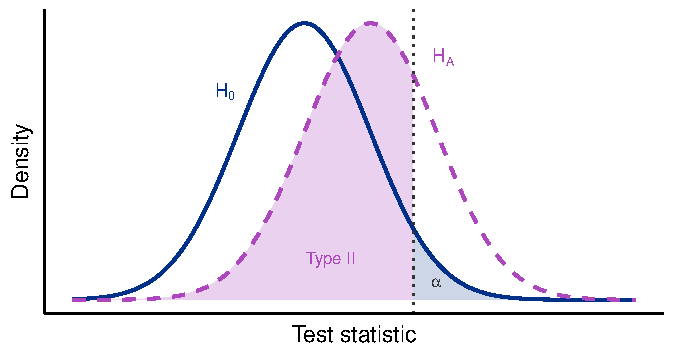
\includegraphics[keepaspectratio,alt={Schematic density plot illustrating a large type II error region. The null distribution H0 is a solid dark-blue bell curve centered at zero. The alternative distribution HA is a dashed purple bell curve centered slightly to the right, heavily overlapping H0. A vertical dotted line marks the rejection threshold. The large purple-shaded area under HA to the left of the threshold is the type II error region, labeled Type II. The small blue-shaded area under H0 to the right of the threshold is labeled alpha. When the alternative is close to the null, most of HA falls in the fail-to-reject zone, so power is low.}]{L12_files/figure-beamer/fig-typeII-large-1.pdf}}

}

\caption{\label{fig-typeII-large}Large type II error region when the
alternative is close to the null.}

\end{figure}%
\end{column}

\begin{column}{0.5\linewidth}
Small type II error region:

\begin{figure}

\centering{

\pandocbounded{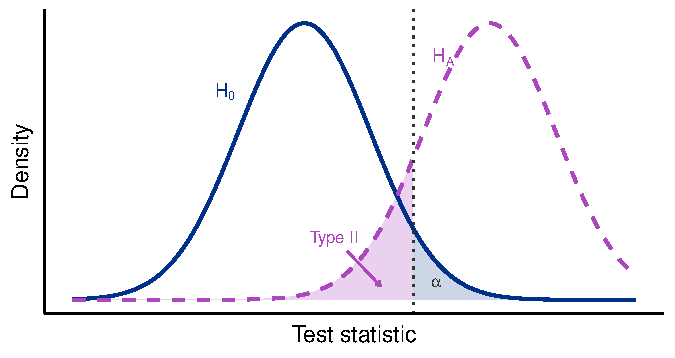
\includegraphics[keepaspectratio,alt={Schematic density plot illustrating a small type II error region. The null distribution H0 is a solid dark-blue bell curve centered at zero. The alternative distribution HA is a dashed purple bell curve centered far to the right, with almost no overlap with H0. A vertical dotted line marks the rejection threshold. The small purple-shaded sliver under HA to the left of the threshold is labeled Type II with an arrow. Almost all of the HA distribution lies to the right of the threshold, indicating high power.}]{L12_files/figure-beamer/fig-typeII-small-1.pdf}}

}

\caption{\label{fig-typeII-small}Small type II error region when the
alternative is far from the null.}

\end{figure}%
\end{column}
\end{columns}
\end{frame}

\begin{frame}{Power: Estimator Distribution}
\protect\phantomsection\label{power-estimator-distribution}
\begin{columns}[T]
\begin{column}{0.5\linewidth}
Parameter assumption and ``best estimator'' distribution:

\begin{figure}

\centering{

\pandocbounded{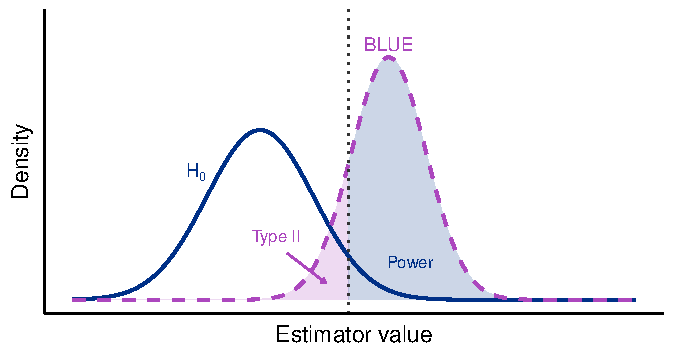
\includegraphics[keepaspectratio,alt={Schematic density plot illustrating high power from the best linear unbiased estimator. The null distribution H0 is a solid dark-blue bell curve centered at zero. The BLUE sampling distribution is a narrow dashed purple bell curve centered to the right of the rejection threshold at 1.645, reflecting its low variance and tall narrow shape. The small purple-shaded region under BLUE to the left of the threshold is labeled Type II. The large blue-shaded region to the right is labeled Power. Because BLUE has minimum variance, its distribution is concentrated to the right of the threshold, yielding high power.}]{L12_files/figure-beamer/fig-power-blue-1.pdf}}

}

\caption{\label{fig-power-blue}High power using the best linear unbiased
estimator (minimum variance).}

\end{figure}%
\end{column}

\begin{column}{0.5\linewidth}
Parameter assumption and other estimator distribution:

\begin{figure}

\centering{

\pandocbounded{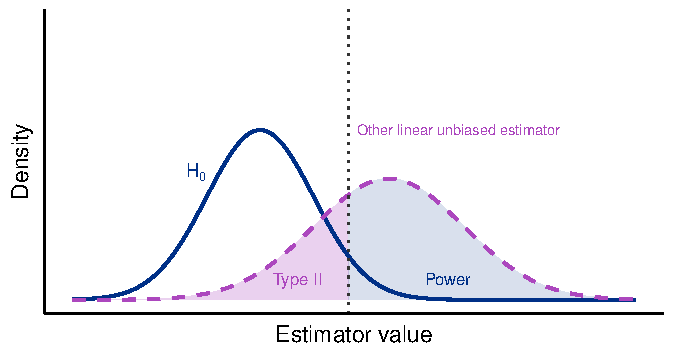
\includegraphics[keepaspectratio,alt={Schematic density plot illustrating low power from a higher-variance linear unbiased estimator. The null distribution H0 is a solid dark-blue bell curve centered at zero. The other linear unbiased estimator\textquotesingle s sampling distribution is a wide dashed purple bell curve centered at the same true parameter value as BLUE, but with higher variance giving a shorter and wider shape. The large purple-shaded region to the left of the threshold is labeled Type II. The smaller blue-shaded region to the right is labeled Power. Because this estimator has higher variance than BLUE, its wider spread places more probability mass in the fail-to-reject region, yielding lower power despite having the same center.}]{L12_files/figure-beamer/fig-power-other-1.pdf}}

}

\caption{\label{fig-power-other}Lower power using a higher-variance
linear unbiased estimator with the same center as BLUE.}

\end{figure}%
\end{column}
\end{columns}
\end{frame}

\begin{frame}{Multiple Hypothesis Testing}
\protect\phantomsection\label{multiple-hypothesis-testing}
\textbf{NOT ON EXAM}

For a single test, we know that \(\Pr(\text{Type I})=\alpha\). If we ran
20 tests in a row, however, we would expect that (on average) one of
those tests yielded a \emph{spurious result} - a Type I error. Although
we will not dig into the methodology in this class, we should consider
additional measures to employ when we are doing many individual tests on
the same sample of data to account for the fact that some of our results
may be false positives.

These \textbf{multiple hypothesis corrections} will be used to show the
robustness of our results when we have to run many tests and are worried
that our probability of a type I error has compounded to a worryingly
large amount.
\end{frame}

\section{End of lecture material}\label{end-of-lecture-material}

\begin{frame}{Knowledge Check 12}
\protect\phantomsection\label{knowledge-check-12}
Consider a test for some parameter \(\theta\) (e.g.~\(\beta_2\)) with
\[H_0:\theta=0\] \[H_A:\theta\neq0\]

Suppose we know that the probability of rejecting \(H_0\) is 0.10 when
\(\theta=0\) and 0.75 when \(\theta\neq0\). Please give:

\begin{enumerate}
[a)]
\item
  The size of the test
\item
  The probability of a type I error
\item
  The probability of a type II error
\item
  The power of the test
\end{enumerate}

Suppose \(n\) is fixed. What could we do to ensure our test is as
well-powered as possible?
\end{frame}




\end{document}
